% todo - biologicke pojmy (ale nie vela) definovat hlavne informaticky problem
% obrazok zarovnania - sekvencie, okno, anotacie
% menej slovies - doplnit pri prednasani

% ak budem mať CRF tak porovnanie CRF a HMM - pozret rydzikovu prezentaciu

% Motivacia, ine vysledky
% Ohurit komisiu
% Urobili vela prace, Nebolo to lahke


\documentclass[xcolor=dvipsnames, compress, 12pt, t]{beamer}
\usepackage[utf8]{inputenc}
\usepackage[slovak]{babel}
\usepackage{lmodern}
\usepackage[T1]{fontenc}
\usepackage{amsfonts}
\usepackage{amssymb}
\usepackage{amsthm}
\usepackage{amsmath}
\usepackage{epsfig}
\usepackage{wrapfig}
\usepackage{caption}
\usepackage{subcaption}
\usepackage{url}
\usepackage{hyperref}
\usepackage{multicol}

\usecolortheme[named=Green]{structure}
\usetheme{Dresden}
\setbeamertemplate{navigation symbols}{}
\usebackgroundtemplate{
\includegraphics[width=\paperwidth, height=\paperheight]{images/bg.png}}
\setbeamercovered{transparent}

% \setbeamertemplate{footline}[frame number]
% \setbeamertemplate{items}[ball]
% \setbeamertemplate{blocks}[rounded][shadow=true]
% \useoutertheme{umbcfootline}

% \AtBeginSection[]{
% \frame<beamer>{

%     \ifpdf
%       \pdfbookmark[0]{Contents}{toc}
%     \fi
%     \frametitle{Obsah}
%     \setcounter{tocdepth}{2}
%     \tableofcontents[currentsection,subsections,hideothersubsections]

% }
% }

% Show frame number in footbar
\setbeamertemplate{footline}%{miniframes theme}
  {%
    \begin{beamercolorbox}[colsep=1.5pt]{upper separation line foot}
    \end{beamercolorbox}
    \begin{beamercolorbox}[ht=2.5ex,dp=1.125ex,%
      leftskip=.3cm,rightskip=.3cm plus1fil]{author in head/foot}%
      \leavevmode{\usebeamerfont{author in head/foot}\insertshortauthor}%
      \hfill%
      {\usebeamerfont{institute in head/foot}\usebeamercolor[fg]{institute in head/foot}\insertshortinstitute}%
    \end{beamercolorbox}%
    \begin{beamercolorbox}[ht=2.5ex,dp=1.125ex,%
      leftskip=.3cm,rightskip=.3cm plus1fil]{title in head/foot}%
      {\usebeamerfont{title in head/foot}\insertshorttitle} \hfill     \insertframenumber /\inserttotalframenumber %
    \end{beamercolorbox}%
    \begin{beamercolorbox}[colsep=1.5pt]{lower separation line foot}
    \end{beamercolorbox}
  }

% items enclosed in square brackets are optional; explanation below
\title{Zarovnávanie sekvencií s~použitím metód klasifikácie}
\subtitle{
\vspace{0.5cm}
\small Diplomová práca
}
\author[Michal Hozza]{\small Bc. Michal Hozza \\ \vspace{1cm} \footnotesize \textbf{Vedúci práce:} Mgr. Tomáš Vinař, PhD. \\ \textbf{Konzultant:} Mgr. Michal Nánási\\ \vspace{.5cm}}
\institute[FMFI UK \insertshortdate]{
  Fakulta matematiky, fyziky a informatiky,
  Univerzita Komenského, Bratislava\\
}
\date[\the\year]{\footnotesize \today}

\newcommand{\lenitem}[2][.6\linewidth]{\parbox[t]{#1}{\strut #2\strut}}

\begin{document}

%--- the titlepage frame -------------------------%
\begin{frame}[plain]
  \titlepage
\end{frame}

%--- the presentation begins here ----------------%

\begin{frame}{Obsah}
  \transdissolve[duration=0.1]
  \begin{multicols}{2}
  \tableofcontents
  \end{multicols}
\end{frame}


\section{Úvod}
\subsection{Cieľ}
\begin{frame}{Cieľ}
  % \transdissolve
  \begin{itemize}
  \item Cieľom práce je vytvoriť nové metódy na korekciu zarovnaní biologických sekvencií na základe prídavnej informácie.
  \item Integrácia tejto informácie bude zabezpečená pomocou techník využívaných na klasifikáciu v~strojovom učení.
  \end{itemize}
\end{frame}


\subsection{Zarovnávanie sekvencií}
\begin{frame}{Zarovnávanie sekvencií}
Kľúčové problémy:
  \begin{itemize}
    \pause
    \item Aké typy zarovnávania by sme mali uvažovať
    \pause
    \item Skórovací systém, ktorý použijeme na ohodnotenie zarovnania a trénovanie
    \pause
    \item Algoritmus, ktorý použijeme na hľadanie optimálneho alebo dobrého zarovnania podľa skórovacieho systému
    \pause
    \item Štatistická významnosť zarovnania.
  \end{itemize}
\end{frame}

\section{Modely a Existujúce riešenia}
\subsection{Modely}
\begin{frame}{Modely}
Generatívny:
\begin{itemize}
\item sa snaží modelovať proces, ktorý generuje dáta ako pravdepodobnosť $P(X,Y,Z)$
\item rozložíme ju pomocou nezávislých predpokladov na procese $\longrightarrow$ obmedzujúce
\end{itemize}
\pause
Diskriminačný
\begin{itemize}
\item priamo odhaduje $P(Z|X,Y)$ alebo prislúchajúcu diskriminačnú funkciu, a preto sa zamerá na podstatnú časť problému odhadu
\item Nepotrebuje nezávislosť $\longrightarrow$ silnejšie
\end{itemize}
\end{frame}


% ToDo - lepsie popisat existujuce modely
\subsection{Príbuzné témy}
\begin{frame}{Príbuzné témy (existujúce riešenia)}
  \begin{itemize}
    \item Problém inverzného zarovnania
    \pause
    \item Support vector training of protein alignment models
    \begin{itemize}
      \item Support Vector Machine (SVM)
      \item Umožňuje trénovať pomocou rôznych účelových funkcií
    \end{itemize}
    \pause
    \item Contralign: Discriminative training for protein sequence alignment.
    \begin{itemize}
      \item Conditional Random Fields (CRF)
      \item Neumožnuje trénovať pomocou rôznych účových funkcií
    \end{itemize}
  \end{itemize}
\end{frame}


\section{Naše riešenia}
\subsection{Odlišnosti nášho riešenia}
\begin{frame}{Odlišnosti nášho riešenia}
  \begin{itemize}
    \item Korekcia existujúcich zarovnaní
    \begin{itemize}
      \item Použitie súbežne s~existujúcimi zarovnávačmi
    \end{itemize}
    \pause
    \item Rôzne modely využitia klasifikátora
    \pause
    \item Rôzne metódy trénovania
    \pause
    \item Možnosť učenia bez učiteľa
    \pause
    \item Iný klasifikátor
    \begin{itemize}
      \item možno porovnanie viac rôznych klasifikátorov
      \item pípadne abstrakcia od klasifikátora
    \end{itemize}
  \end{itemize}
\end{frame}


\subsection{Simulátor}
\begin{frame}{Simulátor}
  \begin{itemize}
    \item Model určený na prvotné experimenty
    \item Program simuluje evolúciu
    \begin{itemize}
      \item Generovanie dvojice postupností so správnym zarovnaním
      \item Generovanie dodatočej informácie
      \item Simulácia mutácie a delécie
    \end{itemize}
  \end{itemize}
\end{frame}

%ToDo: Obrázok
\subsection{Modely}
\begin{frame}{Základný model}
  \mbox{}\hfill\raisebox{-\height}[0pt][0pt]{
   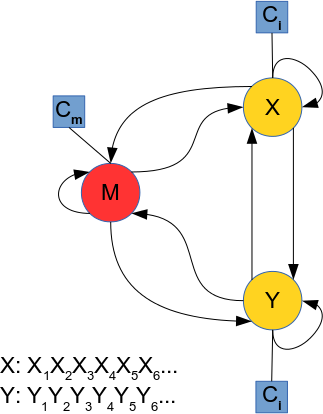
\includegraphics[width=.30\textwidth]{images/zakladny_model}
   }
  \vspace*{-\baselineskip}

  \begin{itemize}
    \item \lenitem{3 stavový HMM}
    \begin{itemize}
      \item \lenitem{Match}
      \item \lenitem{Insert X, Insert Y}
    \end{itemize}
    \item \lenitem{Klasifikátor vidí okolie báz rozšírené o~anotácie}
    \pause
    \item \lenitem{V~HMM sa trénujú iba tranzície, klasifikátory sa trenujú zvlášť}
    \item Viterbiho algoritmus %todo vyzuitie okolia luca
    \begin{itemize}
      \item \lenitem{namiesto tabuľky emisných pravdepodobnosti, máme výstup z~natrénovaného klasifikátora}
      \item Problém výstupy z~klasifikátora nesumujú do 1, čiže model nie je celkom korektný
    \end{itemize}
  \end{itemize}
\end{frame}

\begin{frame}{Distribúcia výstupu z~klasifikátora}{Match stav}
\begin{figure}[hbtp]
    \centering
    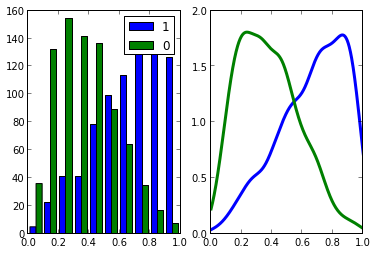
\includegraphics[height=0.5\textheight]{images/clf_m_test.png}
    \caption{Distribúcia výstupu klasifikátora pre zarovnané (modrá) a nezarovnané (zelená) pozície. Klasifikátor pre match stav s~anotáciou a oknom veľkosti 5 (testovacia množina)}
\end{figure}
\end{frame}

\begin{frame}{Distribúcia výstupu z~klasifikátora}{Insert stav}
\begin{figure}[hbtp]
    \centering
    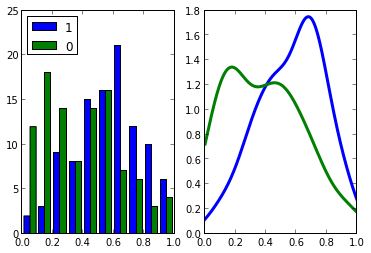
\includegraphics[height=0.5\textheight]{images/clf_i_test.png}
    \caption{Distribúcia výstupu klasifikátora pre zarovnané pozície (zelená) a pozície zarovnané k~medzere (modrá). Klasifikátor pre insert stav s~anotáciou a oknom veľkosti 5 (testovacia množina)}
\end{figure}
\end{frame}


%ToDo: Obrázok
\begin{frame}{Model s~klasifikátorovou páskou}
  \mbox{}\hfill\raisebox{-\height}[0pt][0pt]{
   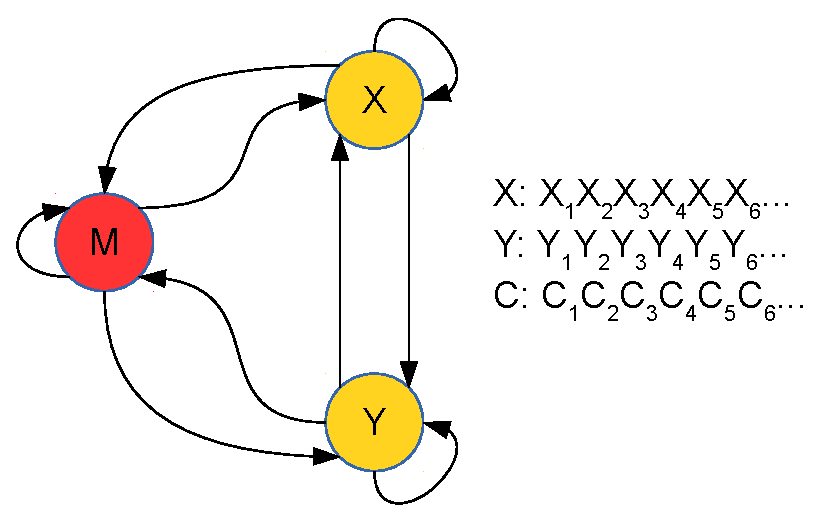
\includegraphics[width=.30\textwidth]{images/model_clf_paska}
   }
  \vspace*{-\baselineskip}
  \begin{itemize}
    \item \lenitem{Opäť rovnaký 3 stavový HMM}
    \item \lenitem{Okrem 2 sekvencií máme ešte pásku s~výstupom z~klasifikátora}
    \item \lenitem{Model teda emituje trojicu - dve písmená zo sekvencií (alebo jedno a pomlčku) a výstup z~klasifikátora}
    \pause
    \item \lenitem{Tento model je narozdiel od predošlého korektný}
    \item \lenitem{Trénujú sa aj prechodové aj emisné pravdepodobnosti}
    \item Pre jednoduchosť budeme emisie výstupu klasifikátora aproximovať pomocou normálneho rozdelenia s~natrénovanými parametrami
  \end{itemize}
\end{frame}

\begin{frame}{Distribúcia výstupu z~klasifikátora}{Match stav - AA}
\begin{figure}[hbtp]
    \centering
    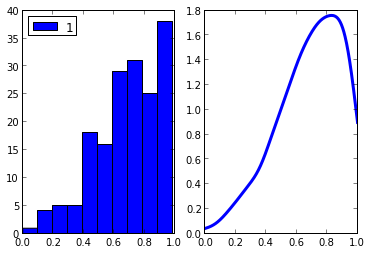
\includegraphics[height=0.55\textheight]{images/distr_aa.png}
    \caption{Distribúcia výstupu klasifikátora pre match stav v~prípade báz AA zarovnaných k~sebe. Klasifikátor s~anotáciou a oknom veľkosti 5 (testovacia množina)}
\end{figure}
\end{frame}

\begin{frame}{Distribúcia výstupu z~klasifikátora}{Match stav - AC}
\begin{figure}[hbtp]
    \centering
    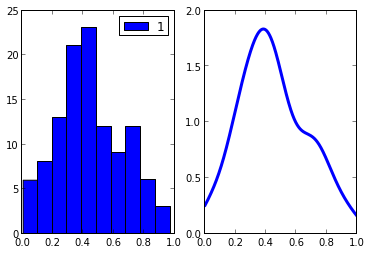
\includegraphics[height=0.55\textheight]{images/distr_ac.png}
    \caption{Distribúcia výstupu klasifikátora pre match stav v~prípade báz AC zarovnaných k~sebe. Klasifikátor s~anotáciou a oknom veľkosti 5 (testovacia množina)}
\end{figure}
\end{frame}

%ToDo: Obrázok
% \begin{frame}{Kombinovaný model}
%   \begin{itemize}
%     \item 3 stavový HMM
%     \begin{itemize}
%       \item Match
%       \item Insert X
%       \item Insert Y
%     \end{itemize}
%     \pause
%     \item Viterbiho algoritmus
%     \begin{itemize}
%     \item pravdepodobnosti získané z natrénovaného klasifikátora
%   \end{itemize}
%   \pause
%   \item rozšírenie sekvencií o anotácie
%   \end{itemize}
% \end{frame}


% \begin{frame}{CRF}
%   \begin{itemize}
%     \item 3 stavový HMM
%     \begin{itemize}
%       \item Match
%       \item Insert X
%       \item Insert Y
%     \end{itemize}
%     \pause
%     \item Viterbiho algoritmus
%     \begin{itemize}
%     \item pravdepodobnosti získané z natrénovaného klasifikátora
%   \end{itemize}
%   \pause
%   \item rozšírenie sekvencií o anotácie
%   \end{itemize}
% \end{frame}

% \subsection{Klasifikátor}
% \begin{frame}{Klasifikátor}
% Random Forest
%   \begin{itemize}
%     \item Zložený z klasifikačných (rozhodovacích) stromov
%     \item Stromy hlasujú o výsledku
%   \end{itemize}
%   \vspace{.5cm}
%   \begin{center}
%   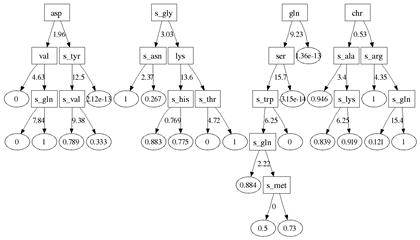
\includegraphics[width=.5\textwidth]{images/random_forest_thumb.png}
%   \end{center}
% \end{frame}


\section{Výsledky}
\subsection{Metódy vyhodnocovania}
\begin{frame}{Metódy vyhodnocovania}{Kontrola tranzitivity}
Ako základnú mieru úspešnosti nášho algoritmu budeme brať kontorlu tranzitivity
  \begin{itemize}
    \item Použijeme 3 párové zarovnania 3 sekvencií (každá s~každou)
    \item Spojíme prvé 2 zarovnania do nového zarovnania
    \item Porovnáme percentuálne zhody nového s~tretím zarovnaním
  \end{itemize}
  % TODO obrazok
\end{frame}

\subsection{Simulované dáta}
\begin{frame}{Dodatočné informácie}
  \begin{itemize}
    \item Stopa s~informáciou, či daná pozícia je súčasťou génu
    \item Ukazuje sa, že dodatočné informácie dokážu pomôcť klasifikátoru v~lepšej klasifikácii`
  \end{itemize}
\end{frame}

% \begin{frame}{Dodatočné informácie}
% \begin{figure}[hbtp]
%     \centering
%     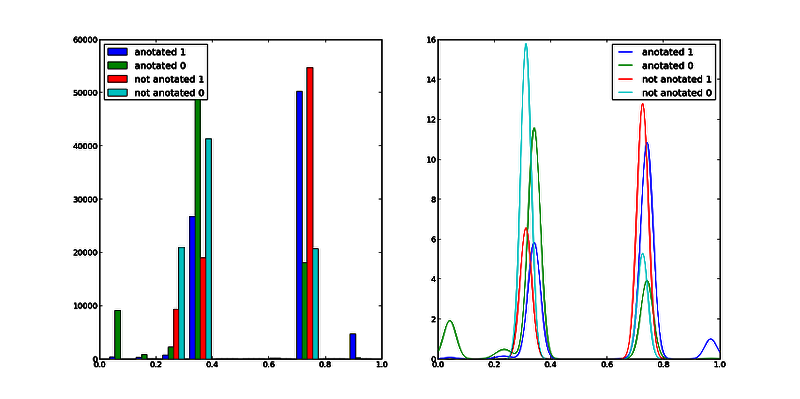
\includegraphics[width=\textwidth]{images/porovnanie_s1w1testset.png}
%     \caption{Porovnanie distribúcie pravdepodobností bez anotácie a s anotáciou (100000 báz, okno veľkosti 1, testovacia množina)}
%     \label{fig:porovnanie_s1w1testset.png}
% \end{figure}
% \end{frame}

% \begin{frame}{Väčšie okno}
%   \begin{itemize}
%     \item Väčšie okno sa prejaví vo väčšom množstve \textit{vlastností}, čo
%     \item Pri malom množstve doplnkovej informácie má výrazný vplyv
%     \item Pri väčšom množstve doplnkovej informácie ich znásobuje
%   \end{itemize}
% \end{frame}

% \begin{frame}{Väčšie okno}
% \begin{figure}[hbtp]
%     \centering
%     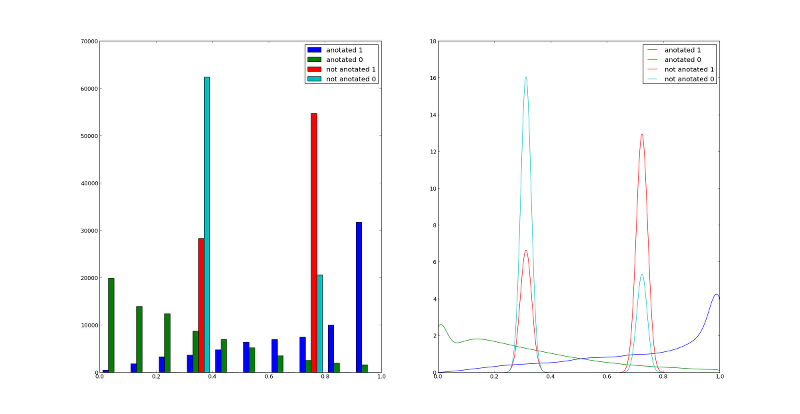
\includegraphics[width=0.9\textwidth]{images/porovnanie_s1w5vsw1testset.png}
%     \caption{Porovnanie distribúcie pravdepodobností bez anotácie a oknom veľkosti 1 a s anotáciou s oknom veľkosti 5 (100000 báz, testovacia množina)}
%     \caption{s1w5vsw1testset}
%     \label{fig:porovnanie_s1w5vsw1testset.png}
% \end{figure}
% \end{frame}



\begin{frame}{Výsledky}
  \begin{itemize}
    \item Aktuálne len na simulovaných dátach
    \item Kontrola tranzitivity:
    \begin{itemize}
      \item Referenčný model (3-stavový HMM bez klasifikátora) --~40\%
      \item Náš základný model (s~1~anotáciou a oknom veľkosti 1) --~\textbf{46\%}
      \item Náš základný model (s~1~anotáciou a oknom veľkosti 5) --~\textbf{46\%}
      \item Model s~klasifikátorovou páskou -- ešte nie je dokončený.
    \end{itemize}
  \end{itemize}
\end{frame}

\section{}
\begin{frame}{Najbližšie plány}
  \begin{itemize}
    \item Dorobiť ostatné modely
    \item Urobiť experimenty na reálnych dátach
    \item Experimenty s~deravým oknom, poprípade iné
    \item V~prvom modeli CRF namiesto HMM?
  \end{itemize}
\end{frame}

\begin{frame}[plain, c]
  \transdissolve[duration=5]
  \begin{center}
  \textbf{\color{Green} \LARGE Ďakujem za pozornosť!}
  \end{center}
\end{frame}


\end{document}
